\chapter{Numerical Analysis}
\label{anexo-na}

\section{Lagrange interpolation}
\label{anexo-interp}
Given real numbers, called nodes, $x_0< x_1 < \ldots< x_m$, we define the $k$-th Lagrange polynomial by
\begin{equation*}
	L_k(x) = \prod_{j=0, j \neq k}^{m}\frac{x-x_j}{x_k-x_j}.
\end{equation*}
They satisfy $L_k(x_j) = \delta_{kj}$, where  $\delta_{kj}$ is the Kronecker delta.
Given a function $f$ defined at the nodes $x_j$, its interpolating polynomial of 
degree $m$ is given by:
\begin{equation*}
	P_m(x) = \sum_{k=0}^{m} f(x_k)L_k(x).
\end{equation*}
Indeed, this polynomial interpolates $f$ since $P_m(x_j) = f(x_j)$.
It is well known that $P_m$ always exists and is unique. Besides that, we have the following error formula
for Lagrange interpolation.
\begin{thrm}
	\label{anexo-interp-error1}
	Let $f \in \mathcal{C}^{m+1}(\mathbb{R})$.
	Then, then there is $\xi$ in the smallest interval containing $x_0, \ldots, x_m, x$ such that:
	\begin{equation}
		f(x)-P_m(x) = \omega(x)\frac{f^{(m+1)}(\xi)}{(m+1)!},
	\end{equation}
	where $\omega(x) = (x-x_0)(x-x_1) \ldots (x-x_m)$.
\end{thrm}
\begin{proof}
	See \citet[Theorem~2.1.4.1. on \pno~49]{stoer:2002}.
\end{proof}

\section{Numerical integration}
\label{anexo-numint}
\begin{thrm}[Leibniz integral rule]
	\label{anexo-numint-lr}
   If $f$...
	\begin{equation*}
	\frac{d}{dx}\int_{a}^{x}f(x,t) \,dt =
   f\big(x, x\big)+
	\int_{a}^{x}\partial_x f(x,t) \,dt
	\end{equation*}
\end{thrm}
\begin{proof}
	See \citet[\pno~143]{courant:1999}.
\end{proof}


The following mean value theorem for integrals is a very useful tool 
when working with numerical integration errors.
\begin{thrm}[Mean value theorem for integrals]
	\label{anexo-numint-mv}
	If $f \in \mathcal{C}([a,b])$, and $g$ is a integrable function in $[a,b]$
	whose sign does not change in $[a,b]$,
	then there exists $c \in ]a,b[$ such that
	\begin{equation*}
		\int_{a}^{b}f(x)g(x) \,dx = f(c)\int_{a}^{b}g(x) \,dx.
	\end{equation*}
\end{thrm}
\begin{proof}
	See \citet[\pno~143]{courant:1999}.
\end{proof}

\subsection{Midpoint rule}
When considering finite-volume schemes, it is useful to compare the average value on a  control volume 
of a function with its value at the  control volume centroid. 
In the following theorems, for the one and two dimensional cases, respectively,
we show that the value of a function at the centroid of a control volume given a second-order approximation to its average value
on the control volume.
\begin{thrm}
	\label{prop-bound-midpoint1d}
	If $f \in \mathcal{C}^2([x_{i-\frac{1}{2}},x_{i+\frac{1}{2}}])$, then 
	\begin{equation}
		\frac{1}{\Delta x}\int_{x_{i-\frac{1}{2}}}^{x_{i+\frac{1}{2}}}{f(x)\,dx}-f(x_i) = C_1 \Delta x^2, 
	\end{equation}
	where $C_1$ is a constant that depends only on $f$, and $x_i = \frac{x_{i+\frac{1}{2}} + x_{i-\frac{1}{2}}}{2}$,
	$\Delta x = x_{i+\frac{1}{2}}-x_{i-\frac{1}{2}}$.
\end{thrm}
\begin{proof}
	From Taylor's expansion, it follows that, for $x \in [x_{i-\frac{1}{2}},x_{i+\frac{1}{2}}]$, we have:
	\begin{equation}
		f(x) = f(x_i) +  f(x_i)(x-x_i) + f''(\xi)\frac{(x-x_i)^2}{2},
	\end{equation}
	for some $\xi$ between $x$ and $x_i$. Therefore:
	\begin{align*}
		\frac{1}{\Delta x} \int_{x_{i-\frac{1}{2}}}^{x_{i+\frac{1}{2}}} {f(x)\,dx} - f(x_i)  
		&= \frac{1}{\Delta x} \int_{x_{i-\frac{1}{2}}}^{x_{i+\frac{1}{2}}} 
		\bigg( f'(x_i)(x-x_i) + f''(\xi)\frac{(x-x_i)^2}{2} \bigg) \,dx \\ 
		&=  \frac{1}{\Delta x} \int_{x_{i-\frac{1}{2}}}^{x_{i+\frac{1}{2}}} 
		f''(\xi)\frac{(x-x_i)^2}{2}  \,dx.
	\end{align*}
	Using the mean value theorem for integrals (see Theorem \ref{anexo-numint-mv}), we have:
	\begin{align*}
		\frac{1}{\Delta x} \int_{x_{i-\frac{1}{2}}}^{x_{i+\frac{1}{2}}} {f(x)\,dx} - f(x_i)  = 
		f''(\eta_i) \frac{1}{\Delta x} \int_{x_{i-\frac{1}{2}}}^{x_{i+\frac{1}{2}}} 
		\frac{(x-x_i)^2}{2}  \,dx = f''(\eta_i)\frac{\Delta x^2}{24}
	\end{align*}	
	for some $\eta_i \in [x_{i-\frac{1}{2}},x_{i+\frac{1}{2}}]$, from which the proposition follows with
	\begin{equation}
		C_1 = \frac{1}{24}f''(\eta_i).
	\end{equation}
\end{proof}

\begin{thrm}
	\label{prop-bound-midpoint2d}
	If $f \in \mathcal{C}^2([x_{i-\frac{1}{2}},x_{i+\frac{1}{2}}]\times [y_{j-\frac{1}{2}},y_{j+\frac{1}{2}}])$, then 
	\begin{equation}
		\frac{1}{\Delta x \Delta y}\int_{x_{i-\frac{1}{2}}}^{x_{i+\frac{1}{2}}}
		\int_{y_{j-\frac{1}{2}}}^{y_{j+\frac{1}{2}}}{f(x,y)\,dx \,dy}-f(x_i,y_j) = C \Delta x^2, 
	\end{equation}
	where $C_1$ is a constants that depends only on $f$, where we assume $x_i = \frac{x_{i+\frac{1}{2}} + x_{i-\frac{1}{2}}}{2}$,
	$y_i = \frac{y_{j+\frac{1}{2}} + y_{j-\frac{1}{2}}}{2}$, $\Delta x = x_{i+\frac{1}{2}}-x_{i-\frac{1}{2}}$,
	$\Delta y= y_{j+\frac{1}{2}}-y_{j-\frac{1}{2}}$ and $\Delta x = \Delta y$.
\end{thrm}
\begin{proof}
	Applying Theorem \ref{prop-bound-midpoint1d} in the $y$ direction, we have
	\begin{align*}
	\int_{y_{j-\frac{1}{2}}}^{y_{j+\frac{1}{2}}} {f(x,y)\,dy} = \Delta y f(x,y_j) +
	\frac{\Delta y^3}{24}\partial_y^2 f(x, \eta_j),
	\end{align*}
	for $\eta_j\in [y_{j-\frac{1}{2}},y_{j+\frac{1}{2}}]$. Hence:
	\begin{align*}
		\int_{x_{i-\frac{1}{2}}}^{x_{i+\frac{1}{2}}}
		\int_{y_{j-\frac{1}{2}}}^{y_{j+\frac{1}{2}}} {f(x,y)\,dx \,dy} = 
		\Delta y \int_{x_{i-\frac{1}{2}}}^{x_{i+\frac{1}{2}}} {f(x,y_j) \,dx}+
		\frac{\Delta y^3}{24}\int_{x_{i-\frac{1}{2}}}^{x_{i+\frac{1}{2}}} {\partial_y^2 f(x, \eta_j)\,dx}.
	\end{align*}
	Applying Theorem \ref{prop-bound-midpoint1d} in the $x$ direction for $y=y_j$, we get
	\begin{align*}
	\int_{x_{i-\frac{1}{2}}}^{x_{i+\frac{1}{2}}} {f(x,y_j)\,dx} = 
	\Delta x {f(x_i,y_j)}+
	\frac{\Delta x^3}{24} {\partial_x^2 f(\xi_i, y_j)\,dx},
	\end{align*}
	for $\xi_i\in [x_{i-\frac{1}{2}},x_{i+\frac{1}{2}}]$. From this, we obtain
	\begin{align*}
	\int_{x_{i-\frac{1}{2}}}^{x_{i+\frac{1}{2}}}
	\int_{y_{j-\frac{1}{2}}}^{y_{j+\frac{1}{2}}} {f(x,y)\,dx \,dy} = 
	\Delta x \Delta y f(x_i,y_j)+
	\frac{\Delta x^3}{24}\int_{x_{i-\frac{1}{2}}}^{x_{i+\frac{1}{2}}} {\partial_x^2 f(\xi_i, y_j)\,dx}+
	\frac{\Delta y^3}{24}\int_{x_{i-\frac{1}{2}}}^{x_{i+\frac{1}{2}}} {\partial_y^2 f(x, \eta_j)\,dx}.
\end{align*}
Using Theorem \ref{anexo-numint-mv}, we obtain the desired formula:
	\begin{align*}
	\int_{x_{i-\frac{1}{2}}}^{x_{i+\frac{1}{2}}}
	\int_{y_{j-\frac{1}{2}}}^{y_{j+\frac{1}{2}}} {f(x,y)\,dx \,dy} = 
	\Delta x \Delta y f(x_i,y_j)+
	\frac{\Delta x^2}{24}\Delta x \Delta y {\partial_x^2 f(\nu_i, y_j)}+
	\frac{\Delta y^2}{24}\Delta x \Delta y {\partial_y^2 f(\theta_i, \eta_j)},
\end{align*}
where $\nu_i, \theta_i\in [x_{i-\frac{1}{2}},x_{i+\frac{1}{2}}]$, recalling that $\Delta x = \Delta y$.
\end{proof}

\begin{corollary}
	\label{anexo-mdp-2d}
	If $f\in \mathcal{C}^2([a,b]\times[c,d])$, and $[a,b]\times[c,d]$ is written
	as the union of the uniformed-spaces control volumes $[x_{i-\frac{1}{2}},x_{i+\frac{1}{2}}] \times  [y_{j-\frac{1}{2}},y_{j+\frac{1}{2}}]$,
	$i,j=1, \ldots, N$,
	with lengths $\Delta x= \Delta y$, we have
	\begin{equation}
	\int_{a}^{b}\int_{c}^{d}
	{f(x,y)\,dx \,dy}-\sum_{i,j=1}^Nf(x_i,y_j) {\Delta x \Delta y} = C_1 \Delta x^2, 
\end{equation}
where $C_1$ depends only on $f$.
\end{corollary}
\begin{proof}
Using Theorem \ref{prop-bound-midpoint2d}, we have:
\begin{align*}
\frac{1}{\Delta x \Delta y}
\int_{a}^{b}\int_{c}^{d} {f(x,y)\,dx \,dy} &=
\frac{1}{\Delta x \Delta y} \sum_{i,j=1}^N
\int_{x_{i-\frac{1}{2}}}^{x_{i+\frac{1}{2}}}
\int_{y_{j-\frac{1}{2}}}^{y_{j+\frac{1}{2}}} {f(x,y)\,dx \,dy}\\
 &= 
\sum_{i,j=1}^N {f(x_i,y_j)} +
\frac{\Delta x^2}{24} \sum_{i,j=1}^N  \bigg({\partial^2_x f(\nu_i,y_j)}+{\partial^2_y f(\nu_i,y_j)}\bigg).
\end{align*}
We notice that
\begin{align*}
{\Delta x \Delta y}
\sum_{i,j=1}^N \bigg(\partial^2_x f(\nu_i,y_j)+\partial^2_y f(\nu_i,y_j)\bigg) = 
\frac{(b-a)(d-c)}{N^2}
\sum_{i,j=1}^N \bigg(\partial^2_x f(\nu_i,y_j)+\partial^2_y f(\nu_i,y_j)\bigg) 
\end{align*}
and we also point that from the inequality
\begin{align*}
	\min{ \big(\partial^2_x f+\partial^2_y f\big)(x,y)} \leq
	\frac{1}{N^2}
	\sum_{i,j=1}^N \bigg(\partial^2_x f(\nu_i,y_j)+\partial^2_y f(\nu_i,y_j)\bigg) 
	\leq \max{ \big(\partial^2_x f+\partial^2_y f\big)(x,y)},
\end{align*}
and with the aid of the intermediate value theorem, we have
\begin{align*}
	\frac{1}{N^2}
	\sum_{i,j=1}^N \bigg(\partial^2_x f(\nu_i,y_j)+\partial^2_y f(\nu_i,y_j)\bigg) 
	= \big(\partial^2_x f+\partial^2_y f\big)(\overline{x},\overline{y}) 
\end{align*}
for some $(\overline{x},\overline{y}) \in [a,b]\times[c,d]$ from which the claim follows.
\end{proof}
\subsection{Multi-step schemes}
Let us consider the following problem: given a function $f \in \mathcal{C}^{m+1}([0,T])$,
a discretization of $[0,T]$ given by $t^n= n\Delta t$, $\Delta t = \frac{T}{N_T}$, for some $N_T \in \mathbb{N}$, we wish
to estimate $\int_{t^n}^{t^{n+1}} f(t)\,dt$ using the values $f(t_{n-k})$, for $k=0,\cdots, m$.
This kind of problem arises, for instance, when we are interested in computing departure points as in Equation \ref{chp-sec-flux:analysis-eq4}.
We can estimate the desired integral by computing the interpolating polynomial of $f(t_{n-k})$, for $k=0,\cdots, m$ and
then integrating this polynomial.
This approach is exactly what is used in multi-step Adams-Bashforth methods.
On the next theorem, we give an expression the error of this approach.

\begin{thrm}
	\label{anexo-numint-adams}
	If $f\in \mathcal{C}^{m+1}([0,T])$, $t^n = n\Delta t$, $n=0, \cdots, N_T$, $\Delta t = \frac{T}{N_T}$ for some 
	$N_T \in \mathbb{N}$, then:
	\begin{equation}
		\label{anexo-numint-eq0}
		\int_{t^n}^{t^{n+1}} f(t)\,dt = \Delta t \sum_{k=0}^{m} \bigg(\int_{0}^{1} L_k(s) \,ds \bigg) f(t_{n-k})
		+ \frac{(\Delta t)^{k+1}}{(m+1)!} f^{(m+1)}(\eta)\int_{0}^{1} \omega(s)\,ds, 
	\end{equation}
	where $w(s) = s(s+1)\cdots(s+m)$, $\eta \in [t^{n-m}, t^{n}]$.
\end{thrm}

\begin{proof}
	We introduce auxiliary functions $\theta(s) = s\Delta t + t_n$, $s \in [-m,1]$ and $g(s) = f(\theta(s))$.
	It is clear that $f(t_{n-k}) = g(-k)$, for $k=-1,0, \cdots, m$.
	Hence, we can write:
	\begin{equation}
		\label{anexo-numint-eq1}
		\int_{t^n}^{t^{n+1}} f(t)\,dt = \Delta t \int_{0}^{1} f(\theta(s))\,ds = \Delta t \int_{0}^{1} g(s)\,ds.
	\end{equation}
	
	Defining the nodes $s_k=-k$ for $k=0, \cdots, m$, it follows from Theorem 
	\ref{anexo-interp-error1} that the interpolating polynomial $P_m$ of $g(s_k)$ satisfies:
	\begin{equation}
		\label{anexo-numint-eq2}
		g(s)-P_m(s) = \omega(s)\frac{g^{(m+1)}(\xi)}{(m+1)!},
	\end{equation}
	where $\xi \in [-m,1]$.
	Substituting Equation \eqref{anexo-numint-eq2} in Equation \eqref{anexo-numint-eq1}, we obtain
	\begin{equation}
		\label{anexo-numint-eq3}
		\int_{t^n}^{t^{n+1}} f(t)\,dt = \Delta t \sum_{k=0}^{m} \bigg(\int_{0}^{1} L_k(s) \,ds \bigg) g(-k)
		+ \frac{\Delta t}{(m+1)!} \int_{0}^{1} g^{(m+1)}(\xi) \omega(s)\,ds.
	\end{equation}
	Since $w(s)$ does not change its sign in $[0,1]$ it follows from Theorem \ref{anexo-numint-mv} that:
	\begin{equation}
		\label{anexo-numint-eq4}
		\int_{t^n}^{t^{n+1}} f(t)\,dt = \Delta t \sum_{k=0}^{m} \bigg(\int_{0}^{1} L_k(s) \,ds \bigg) g(-k)
		+ \frac{\Delta t}{(m+1)!} g^{(m+1)}(\overline{\xi})\int_{0}^{1} \omega(s)\,ds, 
	\end{equation}
	for some $\overline{\xi} \in [-m,1]$. 
	Notice that by the chain rule we get $g^{(m+1)}(s) = (\Delta t)^k f^{(m+1)}(\theta(s))$, therefore
	Equation \eqref{anexo-numint-eq4} in terms of $f$ reads:
	\begin{equation}
		\label{anexo-numint-eq5}
		\int_{t^n}^{t^{n+1}} f(t)\,dt = \Delta t \sum_{k=0}^{m} \bigg(\int_{0}^{1} L_k(s) \,ds \bigg) f(t_{n-k})
		+ \frac{(\Delta t)^{k+1}}{(m+1)!} f^{(m+1)}({\eta})\int_{0}^{1} \omega(s)\,ds, 
	\end{equation}
	where $\eta \in [t^{n-m},t^n]$, which is the desired identity.
\end{proof}

In the following corollaries, we give the explicit formulas for Equation \eqref{anexo-numint-eq5}
for $m=0,m=1,m=2$. This is achieved by computing the terms $\int_{0}^{1} L_k(s) \,ds$ and $\int_{0}^{1} \omega(s)\,ds$,
which are trivial to be computed.
\begin{corollary}
	\label{anexo-numint-col1}
	If $f\in \mathcal{C}^1([0,T])$, $t^n = n\Delta t$, $n=0, \cdots, N_T$, $\Delta t = \frac{T}{N_T}$ for some 
	$N_T \in \mathbb{N}$, then:
	\begin{equation}
		\int_{t^n}^{t^{n+1}} f(t)\,dt = \Delta t  f(t_{n})
		+ \frac{\Delta t^{2}}{2} f^{'}(\overline{t}),
	\end{equation}
	for some $\overline{t} \in [t^n, t^{n+1}]$.
\end{corollary}

\begin{corollary}
	\label{anexo-numint-col2}
	If $f\in \mathcal{C}^2([0,T])$, $t^n = n\Delta t$, $n=0, \cdots, N_T$, $\Delta t = \frac{T}{N_T}$ 
	for some $N_T \in \mathbb{N}$, then:
	\begin{equation}
		\int_{t^n}^{t^{n+1}} f(t)\,dt = \frac{\Delta t}{2} (3f(t_{n}) - f(t_{n-1}) )
		+ \frac{5\Delta t^{3}}{12} f^{(2)}(\overline{t}),
	\end{equation}
	for some $\overline{t} \in [t^{n-1}, t^{n+1}]$.
\end{corollary}

\begin{corollary}
	\label{anexo-numint-col3}
	If $f\in \mathcal{C}^3([0,T])$, $t^n = n\Delta t$, $n=0, \cdots, N_T$, $\Delta t = \frac{T}{N_T}$ 
	for some $N_T \in \mathbb{N}$, then:
	\begin{equation}
		\int_{t^n}^{t^{n+1}} f(t)\,dt = \frac{\Delta t}{12} (23f(t_{n}) - 16f(t_{n-1}) + 5f(t_{n-2}) )
		+ \frac{3\Delta t^{4}}{8} f^{(3)}(\overline{t}),
	\end{equation}
	for some $\overline{t} \in [t^{n-2}, t^{n+1}]$.
\end{corollary}

When using these schemes for and ODE written in its integral form,
$m=0$ gives the classical Euler method; for $m=1$ we get the second-order Adams-Bashforth scheme
and for $m=2$ we have the third-order Adams-Bashforth scheme.

Observe that from the midpoint rule (Theorem  \ref{prop-bound-midpoint1d}),
we can write
\begin{equation}
	\frac{1}{\Delta t}\int_{t^n}^{t^{n+1}} f(t)\,dt = f(t_{n+\frac{1}{2}})
	+ \frac{\Delta t^{2}}{2} f^{'}(\tilde{t}),
\end{equation}
where $t_{n+\frac{1}{2}} = (t_{n+1} + t_{n})/2$ and $\tilde{t} \in [t^n, t^{n+1}]$.
Combining this with Corollary \ref{anexo-numint-col2}, we have the second-order extrapolation formula as follows.
\begin{corollary}
	\label{anexo-numint-col4}
	If $f\in \mathcal{C}^2([0,T])$, $t^n = n\Delta t$, $n=0, \cdots, N_T$, $\Delta t = \frac{T}{N_T}$ 
	for some $N_T \in \mathbb{N}$, then:
	\begin{equation}
		f(t_{n+\frac{1}{2}}) = \frac{3}{2}f(t_{n}) - \frac{1}{2}f(t_{n-1}) + O(\Delta t^2).
	\end{equation}
\end{corollary}


\section{Convergence of 1D FV-SL schemes}
\label{convergence-1dfvsl}
\subsection{Consistency and convergence}
\label{chp-adv1d-sub-CC}
Hereafter, we are going to use the notations introduced in Section \ref{chp-adv1d-sec-not}.
To move towards the convergence of 1D-FV schemes, for  Problem \ref{chp-adv1d-sec2-prob4} we introduce the local truncation error (LTE hereafter)
$\tau_i^n$ following \citet{leveque:2002}:
\begin{equation}
	\label{consistency-1d-eq1}
	Q_i(t^{n+1}) = Q_i(t^n) - \lambda
	\bigg({F}^n_{i+\frac{1}{2}}(Q(t^n),\tilde{u}^n_{i+\frac{1}{2}})-
	{F}^n_{i-\frac{1}{2}}(Q(t^n),\tilde{u}^n_{i-\frac{1}{2}}) \bigg) + \Delta t \tau_i^n.
\end{equation}
We the define $\tau^n \in \mathbb{P}^{N}_{\nu}$, which represent the LTEs at the time-step $n$.
Notice the LTE is obtained by replacing the exact solution in Equation \eqref{1d-fv-scheme}.
Since $Q_i(t^n)$ is the exact solution of Equation \eqref{1d-fvexact-scheme}, 
the LTE may be rewritten as
\begin{align}
	\begin{split}
		\label{consistency-1d-eq2}
		\tau_{i}^n = 
		\frac{1}{\Delta x} \bigg[  \bigg( \frac{1}{\Delta t}\int_{t^{n}}^{t^{n+1}}
		{(uq)}(x_{i+\frac{1}{2}}, t) \,dt - {F}^n_{i+\frac{1}{2}}(Q(t^n),\tilde{u}^n_{i+\frac{1}{2}}) \bigg) +\\
		\bigg( \frac{1}{\Delta t}\int_{t^{n}}^{t^{n+1}}
		{(uq)}(x_{i-\frac{1}{2}}, t) \,dt - {F}^n_{i-\frac{1}{2}}(Q(t^n),\tilde{u}^n_{i-\frac{1}{2}}) \bigg)
		\bigg].
	\end{split}
\end{align}
The LTE gives a measure of how well the 1D-FV scheme approximates the integral form
of the considered conservation law. 
Another interpretation of the LTE is that the LTE gives the error obtained after applying
the scheme for a single time-step using the exact solution.
Now we can define consistency.
\begin{definition}[Consistency]
	\label{chp-adv1d-def-cons}
	Let us consider the framework of Problem \ref{chp-adv1d-sec2-prob4}.
	A 1D-FV scheme is said to be consistency in the $p$-norm if for any sequence of $(\Delta x^{(k)}, \Delta t^{(k)},\lambda)$-discretizations, 
	$k \in \mathbb{N}$, with $\lim_{k\to \infty }{\Delta x^{(k)}} = \lim_{k\to \infty }{\Delta t^{(k)}} = 0$, we have:
	\begin{equation*}
		\lim_{k \to \infty}\bigg[ {\max_{1\leq n\leq N_T^{(k)}}}{\|\tau^n\|_{p,\Delta x^{(k)}}} \bigg] = 0,
	\end{equation*}
	and it is said to be consistent with order $P$ in the $p-$norm if %there 
	%exists a constant 
	%$C$ that does not depend neither on $\Delta t$ nor on $\Delta x$, such that
	\begin{equation*}
		{\max_{1\leq n\leq N_T^{(k)}}}{\|\tau^n\|_{p,\Delta x^{(k)}}} = O(\Delta x^P).
	\end{equation*}
\end{definition}
From Equation \eqref{consistency-1d-eq2}, it follows that we basically need to ensure that 
the numerical flux function $\mathcal{F}^n_{i+\frac{1}{2}}$ converges to the time-averaged flux at edges
when $\Delta x \to 0$ in order to guarantee consistency.
%In Section \ref{chp-adv1d-sec-flux} we shall address how the numerical flux from PPM
%approximates the time-averaged flux at edges.

At last, we define the point-wise error at time-step $n$ by:
\begin{equation*}
	E_i^n = Q_i(t^n) - Q_i^n, \quad i=1, \ldots, N,
\end{equation*}
and we define the vector of errors by $E^n \in \mathbb{P}^{N}_{\nu}$ with entries $E_i^n$.
\begin{definition}[Convergence]
	\label{chp-adv1d-def-conv}
	Let us consider the framework of Problem \ref{chp-adv1d-sec2-prob4}.
	A 1D-FV scheme is said to be convergent in the $p$-norm if for any sequence of $(\Delta x^{(k)}, \Delta t^{(k)},\lambda)$-discretizations, 
	$k \in \mathbb{N}$, with $\lim_{k\to \infty }{\Delta x^{(k)}} = \lim_{k\to \infty }{\Delta t^{(k)}} = 0$, we have:
	\begin{equation*}
		\lim_{k\to \infty}\bigg[ {\max_{1\leq n\leq N_T^{(k)}}}{\|E^n\|_{p,\Delta x^{(k)}}} \bigg] = 0,
	\end{equation*}
	and it is said to converge with order $P$ in the $p-$norm if
	%there exists a constant 
	%$C$ that does not depend neither on $\Delta t$ nor on $\Delta x$, such that
	\begin{equation*}
		{\max_{1\leq n\leq N_T^{(k)}}}{\|E^n\|_{p,\Delta x^{(k)}}} = O(\Delta x^P).
	\end{equation*}
\end{definition}
Subtracting Equation \eqref{1d-fv-scheme} from Equation \eqref{consistency-1d-eq1} we get
the following equation for the error:
\begin{align}
	\begin{split}
		\label{erroreq-1d-eq2}
		E^{n+1}_i = E^n_i -
		&\lambda
		\bigg[
		\bigg( {F}^n_{i+\frac{1}{2}}(Q(t^n),\tilde{u}^n_{i+\frac{1}{2}}) - {F}^n_{i+\frac{1}{2}}(Q^n,\tilde{u}^n_{i+\frac{1}{2}}) \bigg) \\
		&-\bigg( {F}^n_{i-\frac{1}{2}}(Q(t^n),\tilde{u}^n_{i-\frac{1}{2}}) - {F}^n_{i-\frac{1}{2}}(Q^n,\tilde{u}^n_{i-\frac{1}{2}}) \bigg)
		\bigg] 
		+ \tau_{i}^n \Delta t .
	\end{split}
\end{align}
Notice that if $q,u \in \mathcal{C}^3$, we can rewrite Equation \eqref{consistency-1d-eq2} as:
\begin{align*}
	\begin{split}
		\tau_{i}^n = 
		\bigg[ \frac{1}{\Delta x \Delta t}  \int_{t^{n}}^{t^{n+1}} \int_{x_{i-\frac{1}{2}}}^{x_{i+\frac{1}{2}}}
		{\frac{\partial (uq)}{\partial x}}(x, t) \,dx \,dt - 
		\bigg(\frac{{F}^n_{i+\frac{1}{2}}(Q(t^n),\tilde{u}^n_{i-\frac{1}{2}})-{F}^n_{i-\frac{1}{2}}(Q(t^n),\tilde{u}^n_{i-\frac{1}{2}})}{\Delta x} \bigg)
		\bigg].
	\end{split}
\end{align*}
Using the midpoint rule for integration (Theorem \ref{prop-bound-midpoint1d}) and the mean value theorem for integrals
(Theorem \ref{anexo-numint-mv}), 
we have:
\begin{align}
	\begin{split}
		\label{consistency-1d-eq3}
		\tau_{i}^n 
		&= 
		\bigg[ \frac{1}{\Delta t}  \int_{t^{n}}^{t^{n+1}}
		{\bigg(\frac{\partial (uq)}{\partial x}}(x_i, t) + \frac{\Delta x^2}{24}\frac{\partial (uq)}{\partial x}(\xi, t) \bigg) \,dt - 
		\bigg(\frac{{F}^n_{i+\frac{1}{2}}(Q(t^n),\tilde{u}^n_{i+\frac{1}{2}})
			-{F}^n_{i-\frac{1}{2}}(Q(t^n),\tilde{u}^n_{i-\frac{1}{2}})}{\Delta x} \bigg)
		\bigg] \\
		& = 
		\bigg[ \frac{1}{\Delta t}  \int_{t^{n}}^{t^{n+1}}
		{\frac{\partial (uq)}{\partial x}}(x_i, t) \,dt - 
		\bigg(\frac{{F}^n_{i+\frac{1}{2}}(Q(t^n),\tilde{u}^n_{i+\frac{1}{2}}) - {F}^n_{i-\frac{1}{2}}(Q(t^n),\tilde{u}^n_{i-\frac{1}{2}})}{\Delta x} \bigg)
		\bigg] +  \frac{\Delta x^2}{24}\frac{\partial^3 (uq)}{\partial x^3}(\xi, \overline{t}), 
	\end{split}
\end{align}
for $\xi \in X_i$ and $\overline{t} \in [t^{n},t^{n+1}]$. Therefore, if $q,u \in \mathcal{C}^3$ the scheme is
consistent, if and only if, $\frac{1}{\Delta t}  \int_{t^{n}}^{t^{n+1}} {\frac{\partial (uq)}{\partial x}}(x_i, t) \,dt$
is approximated by 
$\frac{{F}^n_{i+\frac{1}{2}}(Q(t^n),\tilde{u}^n_{i+\frac{1}{2}})) -{F}^n_{i-\frac{1}{2}}(Q(t^n),\tilde{u}^n_{i-\frac{1}{2}})}{\Delta x}$.
This shall be very useful when we consider two-dimensional schemes, where we are going to use the discrete operators to estimate the divergence
of velocity fields.

\subsection{Stability}
\label{chp-adv1d-sub-stability}
In order to define the concept of stability, it is useful to introduce an operator
representation of 1D-FV schemes.
In the context of Problem \ref{chp-adv1d-sec2-prob4}, we define the operators
$\mathcal{H}_{\Delta x,n}: \mathbb{P}^{N}_{\nu} \to \mathbb{P}^{N}_{\nu}$ whose $i$-th entry is given by:
\begin{equation}
	[\mathcal{H}_{\Delta x,n}(Q)]_i = Q_i -
	\lambda \bigg({F}^n_{i+\frac{1}{2}}(Q,\tilde{u}^n_{i+\frac{1}{2}}) 
	- {F}^n_{i-\frac{1}{2}}(Q,\tilde{u}^n_{i-\frac{1}{2}}) \bigg),
\end{equation}
for $i=1, \ldots, N$, $n=0, \ldots, N_T-1$.
Notice that the dependence on $n$ is due to the velocity that may be allowed
to vary with time.
As it is usual, we are assuming periodicity in the entries of $Q$ when 
we apply the operator $\mathcal{H}_{\Delta x,n}$.
Thus, Equation \eqref{1d-fv-scheme} may be rewritten in a vector form by
\begin{equation*}
	Q^{n+1} = \mathcal{H}_{\Delta x,n}(Q^n),
\end{equation*}
and Equation \eqref{consistency-1d-eq1} in a vector form reads
\begin{equation*}
	Q(t^{n+1}) = \mathcal{H}_{\Delta x,n}(Q(t^n)) + \Delta t \tau^n,
\end{equation*}
and the error equation \eqref{erroreq-1d-eq2} is given by
\begin{equation}
	\label{erroreq-1d-eq3}
	E^{n+1} = \mathcal{H}_{\Delta x,n}(Q(t^n)) - \mathcal{H}_{\Delta x,n}(Q^n) +  \Delta t \tau^n.
\end{equation}
The stability theory focus on uniformly bounding the norm of $\mathcal{H}_{\Delta x,n}(Q(t^n)) - \mathcal{H}_{\Delta x,n}(Q^n)$ \citep{leveque:2002}.
We define stability as follows.

\begin{definition}[Stability]
	In the context of Problem  \ref{chp-adv1d-sec2-prob4},
	a 1D-FV scheme is stable in the $p-$norm if for any $(\Delta x, \Delta t, \lambda)$-discretization of $[a,b]\times [0,T]$ we have:
	\begin{equation}
		\|\mathcal{H}_{\Delta x,n}(Q) - \mathcal{H}_{\Delta x,n}(P)\|_{p,\Delta x} \leq (1+\alpha \Delta t)  \|Q-P\|_{p,\Delta x},
	\end{equation}
	for all $Q, P \in \mathbb{R}^{N}_{\nu}$ and $\alpha$ is a constant
	that does not depend neither on $\Delta x$ nor on  $\Delta t$.
\end{definition}
Assuming that the scheme is stable in the $p-$norm, then it follows from Equation \eqref{erroreq-1d-eq3} that:
\begin{align}
	\label{chp-adv1d-sec2-erroreq}
	\begin{split}
		\|E^{n+1}\|_{p,\Delta x} 
		&\leq \|\mathcal{H}_{\Delta x,n}(Q(t^n)) - \mathcal{H}_{\Delta x,n}(Q^n)\|_{p,\Delta x} +  \Delta t \max_{n=1, \ldots, N_T}\|\tau^n\|_{p,\Delta x}\\
		&\leq (1+\alpha \Delta t)\|E^n\|_{p,\Delta x} +  \Delta t \max_{n=1, \ldots, N_T}\|\tau^n\|_{p,\Delta x}\\
		&\leq (1+\alpha \Delta t)^n\|E^0\|_{p,\Delta x} +  \Delta t \max_{n=1, \ldots, N_T}\|\tau^n\|_{p,\Delta x}
		\sum_{k=0}^{n-1} (1+\alpha \Delta t)^k\\
		&\leq e^{\alpha T}(\|E^0\|_{p,\Delta x} + T\max_{n=1, \ldots, N_T}\|\tau^n\|_{p,\Delta x}), \\
	\end{split}
\end{align}
where we used $n \Delta t\leq T $, $T=N\Delta t$ and the inequality $e^t> 1+t$.
When computing the initial average values using the value at the cell centroid, 
the initial error $E^0$ converges to zero provided $q$ is twice continuously differentiable
by Proposition \ref{prop-bound-centroid}.
Therefore, it follows that if the scheme is stable and consistent
then it is convergent. 
Furthermore, if it is stable and consistent with order $P$, then
the convergence order is at least equal to $\min\{{P,2}\}$.
In the case where both the conservation law and $\mathcal{H}_{\Delta x,n}$ are linear,
this result is a particular case of the Lax-Ritchmyer stability and the convergence
is guaranteed by the Lax equivalence theorem \citep{leveque:2002}.
In this Chapter, we are interested only in the linear advection equation.
However, as pointed in Section \ref{chp-adv1d-sec-flux}, the operator $\mathcal{H}_{\Delta x,n}$
may become non-linear when monotonicity constraints are activated.

Notice that, if $\mathcal{H}_{\Delta x,n}$ is linear, then stability is equivalent to require that
\begin{equation*}
	\|\mathcal{H}_{\Delta x,n}\|_{p,\Delta x} \leq 1+ \alpha \Delta t,
\end{equation*}
where
\begin{equation*}
	\|\mathcal{H}_{\Delta x,n}\|_{p,\Delta x} = \sup_{Q\in \mathbb{R}^{\Delta x}} \frac{\|\mathcal{H}_{\Delta x,n}(Q)\|_{p,\Delta x}}{\|Q\|_{p,\Delta x}},
\end{equation*}
is the operator $p$-norm.

For linear operators, we may use the discrete Fourier transform \citep{trefethen:2000}
to estimate the 2-norm of $\mathcal{H}_{\Delta x,n}$. This approach is known as Von Neumann stability analysis.
We define the nodes $\theta_i = i\frac{2\pi}{N}$, $i=1, \ldots, N$, $\Delta \theta = \frac{2\pi}{N}$,
$\theta = (\theta_1, \theta_2, \ldots, \theta_N)$.
The imaginary unit is denoted by $\imath$.
We define $\mathbb{C}^{N}_{\nu}$  similarly as $\mathbb{P}^{N}_{\nu}$.
The Fourier modes $e^{\imath k \theta}] \in \mathbb{C}^{N}_{\nu}$ for $k=1, \ldots, N$, have entries are given by:
\begin{equation*}
	[e^{\imath k \theta}]_i = e^{\imath k\theta_i},\quad \text{for } i=1, \ldots, N.
\end{equation*}
Each $k$ is referred to wavenumber and $\theta_k$ is called  dimensionless wavenumber.
The Fourier modes form an orthogonal basis of $\mathbb{C}^N_{\nu}$ with respect to the 
inner product
\begin{equation*}
	\langle Q, P \rangle = \frac{1}{N}\sum_{i=1}^{N}{Q_i \overline{P_i}},
\end{equation*}
for $P, Q \in \mathbb{C}^{N}_{\nu}$ and $\overline{z}$ denotes the complex conjugate of $z$. 
Given $Q \in \mathbb{P}^{N}_{\nu}$, we may may express it in terms of the Fourier modes
\begin{equation*}
	Q = \sum_{k=1}^{N} a_k e^{\imath k \theta},
\end{equation*}
where $a_k \in \mathbb{C}$. The 2-norm of $Q$ is then given by:
\begin{equation*}
	\|Q\|_{2,\Delta x} = \sqrt{N \sum_{k=1}^{N} |a_k|^2}.
\end{equation*}
The idea of Von Neumann stability analysis is to apply the operator $\mathcal{H}_{\Delta x,n}$ on each Fourier mode and
analyze how it modifies its amplitude.
For ease of analysis, we assume that the velocity is constant, which implies that
the operator $\mathcal{H}_{\Delta x,n}$ has constant coefficients and does not depend on $n$.
For the general case, where the velocity is not constant, the stability
can be ensured using the frozen coefficients method \citep[p.~59]{strikwerda:2004}.
This method boils down to performing multiple times the stability analysis with a constant velocity
being equal to each one of the possible values of the velocity on the grid.
If the scheme is stable for all the possible constant velocities, then stability is ensured.
Since the operator is supposed to be linear with constant coefficients and we
are assuming periodic boundaries conditions, we may write:
\begin{equation*}
	\mathcal{H}_{\Delta x,n}(e^{\imath k \theta}) = \rho(k)  e^{\imath k \theta},
\end{equation*}
where the term $\rho(k)$ is called amplification factor and it is an eigenvalue of $\mathcal{H}_{\Delta x,n}$.
The norm of $\mathcal{H}_{\Delta x,n}(Q)$ is bounded by:
\begin{equation*}
	\|\mathcal{H}_{\Delta x,n}(Q)\|_{2,\Delta x}^2 = N \sum_{k=1}^{N} |a_k|^2 |\rho(k)|^2 \leq 
	\max_{k=1, \ldots, N}{|\rho(k)|}^2 \|Q\|_{2,\Delta x}^2.
\end{equation*}
Therefore:
\begin{equation*}
	\|\mathcal{H}_{\Delta x,n}\|_{2,\Delta x} \leq \max_{k=1, \ldots, N}{|\rho(k)|}.
\end{equation*}
If we show that $\max_{k=1, \ldots, N}{|\rho(k)|} \leq 1 + \alpha \Delta t$, 
with $\alpha$ independent of $\Delta t$, $N$ and $n$, then we ensure the stability of $\mathcal{H}_{\Delta x,n}$.

\subsection{Flux accuracy analysis}
\label{chp2-sub-flux}
With the PPM operator, we can compute the amplification factor by applying it
on each Fourier mode considering the PPM and the hybrid PPM schemes, both without monotonization.
We assume a constant velocity equal to one and $N=100$ (number of control volumes).
In Figure \ref{chp2-fig-amplification} we show the amplification factor for both PPM and hybrid PPM schemes
considering different CFL numbers.
We can observe that both schemes damp most of the Fourier modes for larger $k$, regardless of the CFL number.
Besides that, the hybrid scheme is more effective when reducing the Fourier modes amplitude.
We point out that both schemes are exact when the CFL number is equal to 1.
From this analysis, we can conclude that the PPM and hybrid PPM schemes satisfy the
Von Neumann stability criteria when the CFL restriction is respected.
For an analysis of stability for larger time-steps, we refer to \citet{lauritzen:2007}.
\begin{figure}[ht]
	\centering
	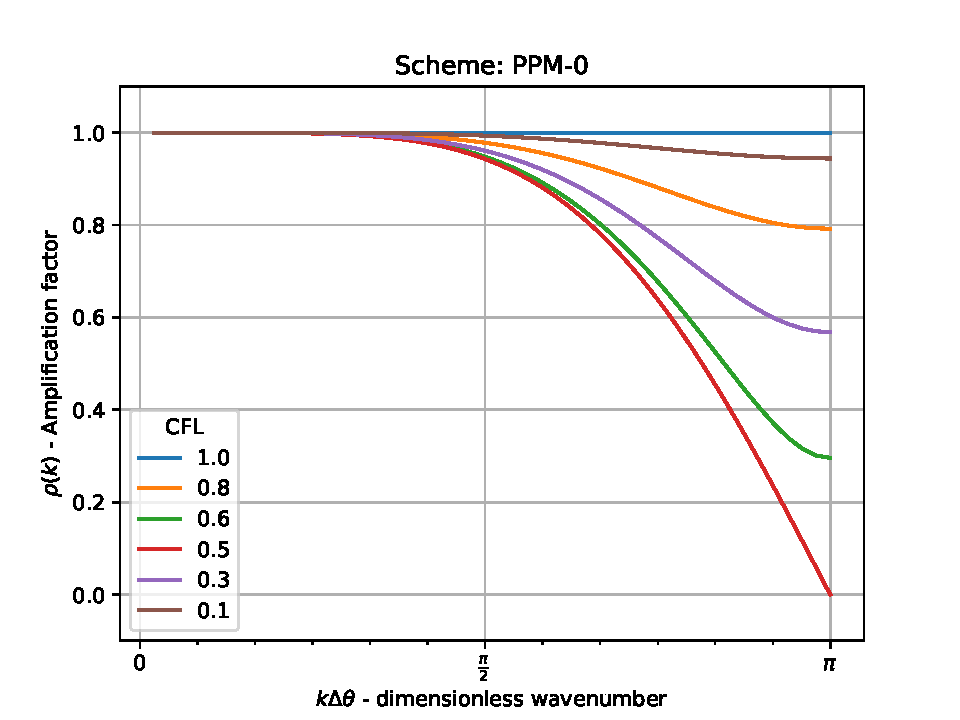
\includegraphics[width=0.49\linewidth]{stability_PPM-0}
	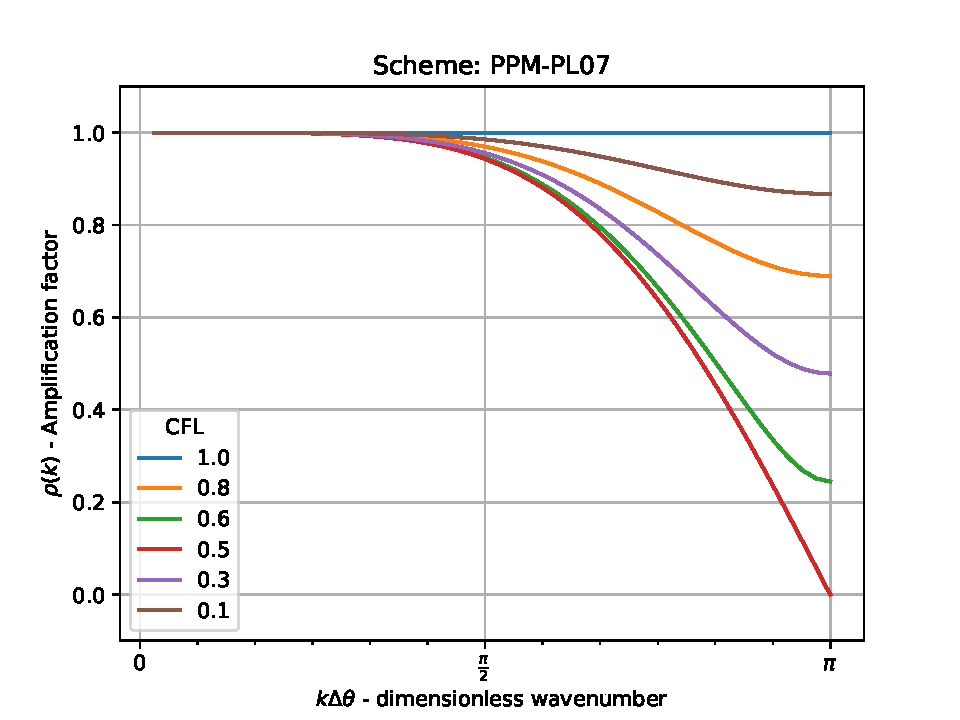
\includegraphics[width=0.49\linewidth]{stability_PPM-PL07}
	\caption{Amplification factor for the PPM (left) and hybrid PPM (right) schemes for different CFL numbers.}
	\label{chp2-fig-amplification}
\end{figure}

\section{Convergence, consistency and stability of 2D-FV schemes}
\label{chp3-CCS}
The notions of convergence, consistency and stability for a 2D-FV schemes
are straightforward from these notions for 1D-FV schemes
(see Subsections \ref{chp-adv1d-sub-CC} and \ref{chp-adv1d-sub-stability}).
Indeed, in the context of Problem \ref{chp3-sec2-prob3}, we define the operators
$\mathcal{H}_{\Delta x ,\Delta y,n}: \mathbb{R}^{N \times M} \to \mathbb{R}^{N \times M}$ whose $(i,j)$ entry is given by:
\begin{align*}
	[\mathcal{H}_{\Delta x ,\Delta y,n}(Q)]_{ij} = Q_{ij} - \Delta t\mathbb{D}_{ij}^n
\end{align*}
for $i=1, \ldots, N$, $j=1, \ldots, M$, $n=0, \ldots, N_T-1$. The 2D-FV is then expressed as
\begin{equation*}
	Q^{n+1} = \mathcal{H}_{\Delta x ,\Delta y,n}(Q^n).
\end{equation*}
The local error truncation $\tau^n \in \mathbb{R}^{N \times M}$ is given by
\begin{equation*}
	Q(t^{n+1}) = \mathcal{H}_{\Delta x ,\Delta y,n}(Q(t^n)) + \Delta t \tau^n.
\end{equation*}
The error equation is given by
\begin{equation}
	E^{n+1} = \mathcal{H}_{\Delta x ,\Delta y,n}(Q(t^n)) - \mathcal{H}_{\Delta x ,\Delta y,n}(Q^n) +  \Delta t \tau^n.
\end{equation}
The stability in the $p$-norm is defined as in the 1D case.
\begin{definition}
	A 2D-FV scheme is stable in the $p-$norm if 
	\begin{equation}
		\|\mathcal{H}_{\Delta x ,\Delta y,n}(Q) - \mathcal{H}_{\Delta x ,\Delta y,n}(P)\|_{p,\Delta x \times \Delta y} \leq (1+\alpha \Delta t)  \|Q-P\|_{p,\Delta x \times \Delta y},
	\end{equation}
	for all $Q, P \in \mathbb{R}^{N\times M}$ and $\alpha$ is a constant
	that does not depend neither on $\Delta x$, $\Delta y$, $\Delta t$ nor on $n$.
\end{definition}
If a 2D-FV scheme is stable in the $p-$norm, similarly to Equation \eqref{chp-adv1d-sec2-erroreq} we have:
\begin{align*}
		\|E^{n+1}\|_{p,\Delta x \times \Delta y} &\leq e^{\alpha T}(\|E^0\|_{p,\Delta x \times \Delta y} + T\max_{n=1, \ldots, N_T}\|\tau^n\|_{p,\Delta x \times \Delta y}).\\
\end{align*}
Again, we point out that from Proposition \ref{prop-bound-centroid-2d}, we have that the initial error $E^0$ shall be second-order accurate.
Consistency is defined as in Definition \ref{chp-adv1d-def-cons} and convergence is defined as in Definition \ref{chp-adv1d-def-conv}.

The Von Neumann analysis can be applied when $\mathcal{H}_{\Delta x ,\Delta y,n}$ is linear, since we are considering periodic boundary conditions.
The idea is the same as in the one-dimensional case, we just apply the operator $\mathcal{H}_{\Delta x ,\Delta y,n}$ on the Fourier modes to obtain
the amplification factor.
We introduce the nodes $\theta_i = i\frac{2\pi}{N}$, $i=1, \ldots, N$, $\Delta \theta = \frac{2\pi}{N}$,
$\theta_i = (\theta_1, \theta_2, \ldots, \theta_N)$, $\phi_j = j\frac{2\pi}{M}$, $j=1, \ldots, M$, $\Delta \phi = \frac{2\pi}{M}$,
$\phi = (\phi_1, \phi_2, \ldots, \phi_M)$.
For $k_1=1, \ldots, N$, $k_2=1, \ldots, M$, the two-dimensional Fourier mode $\boldsymbol{k} = (k_1,k_2)$ from $\mathbb{C}^{N\times M}$ 
has its $(i,j)$ entry given by $[e^{\imath \boldsymbol{k} \theta}]_{ij} = e^{\imath k_1 \theta_i}e^{\imath k_2 \phi_j}$. 
For an analysis of stability for the dimension splitting method, we refer to \citet{lin:1996,lauritzen:2007}.

Notice that if $q,u, v \in \mathcal{C}^3$, we can rewrite the LTE as:
\begin{align*}
	\begin{split}
		\tau_{ij}^n &= 
		\bigg[ \frac{1}{\Delta x \Delta y \Delta t}  \int_{t^{n}}^{t^{n+1}}\int_{x_{i-\frac{1}{2}}}^{x_{i+\frac{1}{2}}} 
		\int_{y_{j-\frac{1}{2}}}^{y_{j+\frac{1}{2}}} {\nabla \cdot (\boldsymbol{u}q)}(x, y, t) \,dy \,dx \,dt 
        -\mathbb{D}_{ij}^n
		\bigg].
	\end{split}
\end{align*}
Using the midpoint rule for integration (Theorem \ref{prop-bound-midpoint2d}), the mean value theorem for integrals
(Theorem \ref{anexo-numint-mv}) and recalling the discrete divergence (Definition \ref{chp3-def-div}), we have:
\begin{align}
	\begin{split}
		\label{consistency-2d-eq}
		\tau_{ij}^n 
		&= \frac{1}{\Delta t}  \int_{t^{n}}^{t^{n+1}}
		{\nabla \cdot (\boldsymbol{u}q)}(x_i, y_j, t)  \,dt - 
		\mathbb{D}^n_{ij} + O(\Delta x^2) + O(\Delta y^2).
	\end{split}
\end{align}
Therefore, in order to investigate the consistency, we may compare how well the discrete divergence approximates the divergence.


